\documentclass{beamer}

\usepackage[brazil]{babel}
\usepackage[utf8]{inputenc}
\usepackage{graphicx}

\usetheme{Warsaw}
\usecolortheme{beetle}

\newcommand{\putat}[3]{\begin{picture}(0,0)(0,0)\put(#1,#2){#3}\end{picture}}

\begin{document}

	\title{Robô Explorador de Ambientes}
	\author{Luis Camargo \newline \  Marcelo Teider \newline \  Matheus Araujo}
	\institute{Orientação: Dra. Myriam Delgado \newline Co-orientação: Dr.Hugo Vieira \newline \newline Universidade Tecnológica Federal do Paraná}

	\date{7 Dez 2011}

	\frame{\titlepage}

	\frame{

		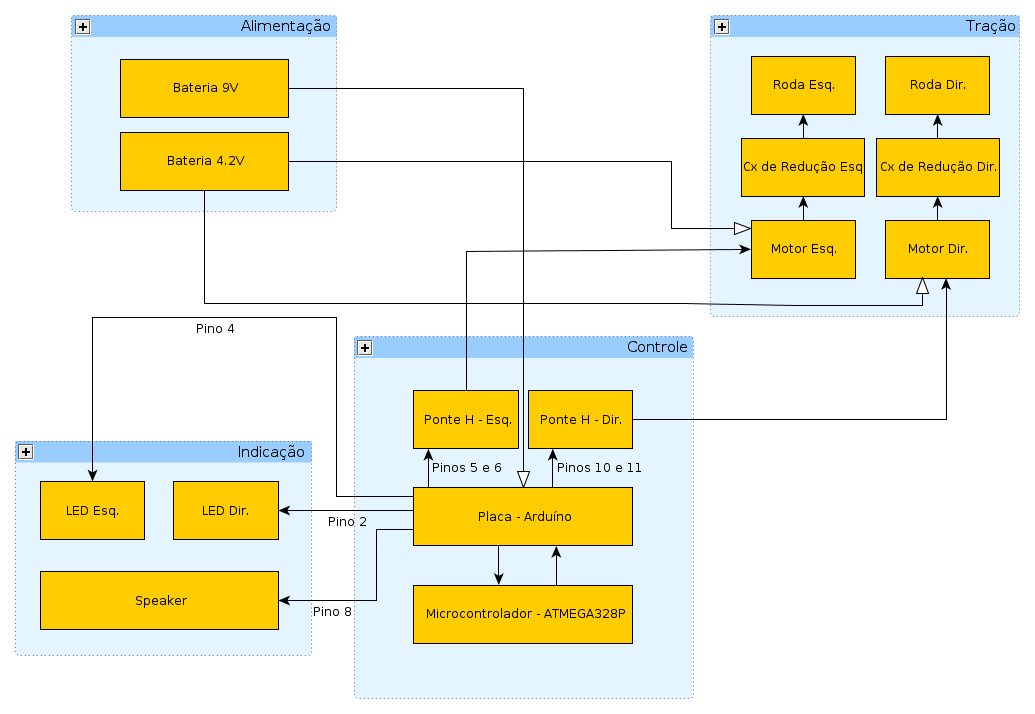
\includegraphics[width=11cm,height=7cm]{images/robo}
	}

	\section{Introdução}
	
	\frame{

		\frametitle{Introdução}
		
		\begin{itemize}
			
			\item \textbf{O que é?}

				\begin{itemize}

					\item Projeto de um robô que explora ambientes em busca de um objeto específico usando uma câmera como sensor.

				\end{itemize}

			\item \textbf{Por quê?}

				\begin{itemize}

					\item Porque é legal!

					\item Robôs exploradores têm diversas aplicações, desde atividades em hospitais a explorações espaciais.

				\end{itemize}
			
		\end{itemize}

	}

	\subsection{Visão Geral}

	\frame{

		\frametitle{Visão Geral}

		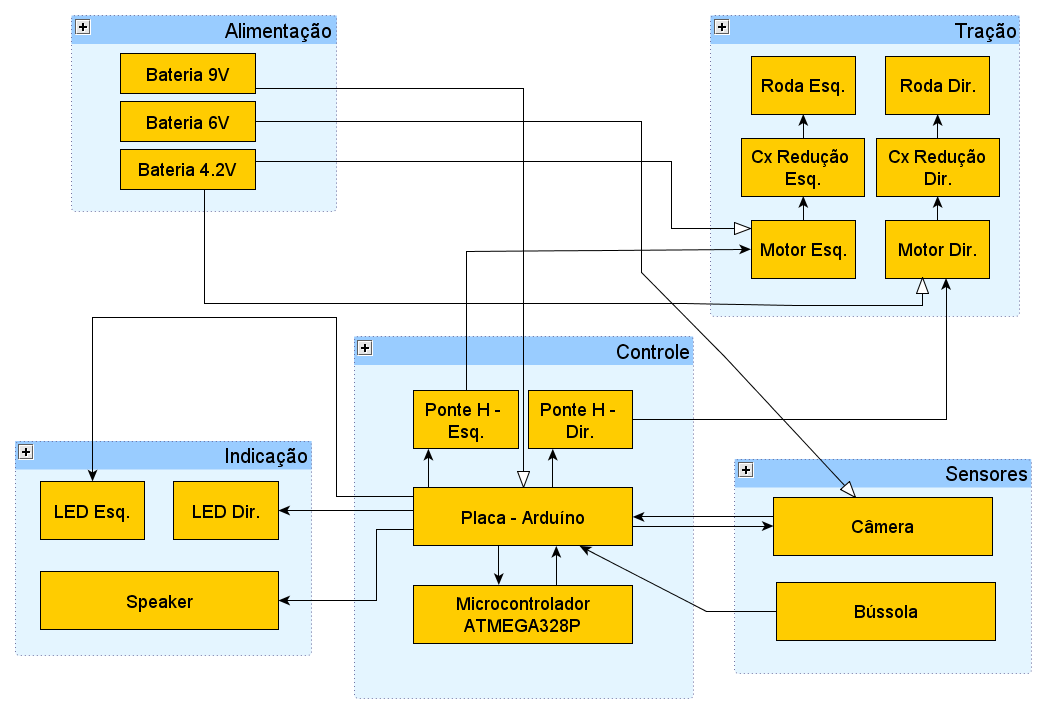
\includegraphics[width=11cm, height=7cm]{images/robo_geral}

	}

		\subsection{Objetivos}

		\frame {

			\frametitle{Objetivo Geral}

			\begin{itemize}

				\item Criar um robô capaz de reconhecer um objeto específico, e posteriormente explorar o ambiente onde se encontra, à procura do objeto.

			\end{itemize}

		}

		\frame{

			\frametitle{Objetivos Parciais}

			\begin{itemize}

				\item Sistema de Controle do Robô

				\item Obter Informações da Bússola

				\item Reconhecimento do Objeto a ser encontrado

				\item Comunicação entre Arduino e Câmera.

				\item Reconhecimento de Pontos de Interesse no ambiente.

				\item Reconhecimento de Obstáculos

				\item Algoritmo de Navegação

			\end{itemize}

		}

	\section{Projeto Mecânico}

		\frame{

			\frametitle{Projeto Mecânico}

			\begin{itemize}

				\item Robô construído no projeto \textbf{Robô Explorador de Labirintos 2D}, Bruno Meneguele, Fernando Padilha e Vinicius Arcanjo, apresentado a esta disciplina no primeiro semestre de 2011.

				\item Foram reutilizados: chassi, motor, caixa de redução, rodas, \textit{Arduino}. 

				\item Os sensores de luz infravermelha foram substituídos pela câmera.

			\end{itemize}

		}


		\subsection{Robô}

			\frame{

				\frametitle{Robô}


				\begin{centering}

					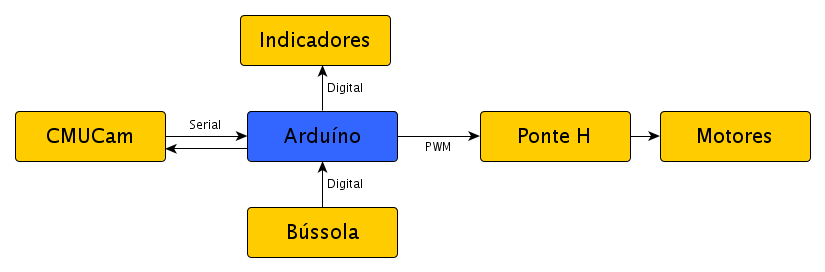
\includegraphics[width=7cm, height=3cm]{images/processo_arduino}

				\end{centering}


				\begin{itemize}


					\item O projeto do robô está centrado no \textit{Arduino} - Ele é o responsável por receber as decisões tomadas pela câmera e atuar sobre os sistemas do robô.

					\item O acionamento dos motores é feito através da Ponte H, que por sua vez é ativada por PWM.

				\end{itemize}

			}

	\section{Sensores}
			
        \subsection{CMUCam}


			\frame{

				\frametitle{CMUCam}

				\putat{200}{-50}{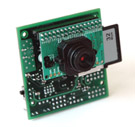
\includegraphics[width=3cm, height=3cm]{images/cmucam}}

				\begin{itemize}

					\item \textit{CMUCam3} - desenvolvida pela \\ \textit{Carmegie Mellon University}.

					\item \textit{Sensor inteligente.}

					\item Busca criar um sistema de visão simples que funcione em sistemas embarcados.

					\item Arquitetura baseada em \textit{ARM7TDMI}, Microprocessador \textit{Philips LPC2106}

				\end{itemize}

			}
                
		
		\subsection{Bússola}

		\frame{

			\frametitle{Bússola}

			\putat{210}{-20}{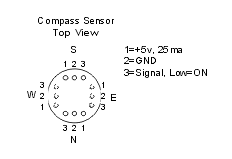
\includegraphics[width=2.75cm, height=2.5cm]{images/bussola1}}
			\putat{210}{-120}{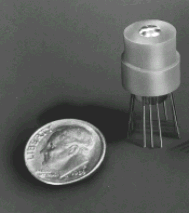
\includegraphics[width=2.75cm, height=2.5cm]{images/bussola2}}

			\begin{itemize}

				\item Apesar de não ter sido utilizada no \\ robô final, a equipe estudou e fez testes \\ com a bússola digital $Dinsmore \  \#1490$.

				\item Ela é capaz de fornecer a orientação \\ geográfica com 45 graus de precisão \\ através de quatro portas TTL.

			\end{itemize}

		}

		\subsection{Comunicação}

			\frame{

				\frametitle{Comunicação}

				\begin{itemize}


					\item Os algoritmos de visão e navegação são executados na \textit{CMUCam}, que deve enviar comandos de movimento para o \textit{Arduino}.

					\item Foi utilizada comunicação serial assíncrona \textit{full-duplex} entre as duas plataformas.

					\item A \textit{CMUCam} envia um \textit{byte} contendo o movimento que deve ser executado pelo robô para o \textit{Arduino} que o interpreta e executa.


				\end{itemize}

			}

    	\section{Exploração}

	
			\frame{

				\frametitle{Exploração}

				\begin{itemize}

					\item No início do projeto, foi proposto um algoritmo de navegação avançado que utilizaria uma percepção local do ambiente e então o exploraria.

					\item No entanto, devido a atrasos nas fases inicias do projeto, não foi possível implementá-lo a tempo desta apresentação.

					\item Foi implementado um algoritmo de navegação que encontra o objeto alvo, desde que ele esteja no campo de visão, e então move o robô até o mesmo.

				\end{itemize}
		
			}

		\subsection{Track-color}


		\frame{
			
			\frametitle{\textit{Track-color}}

			\begin{itemize}

				\item Funcionalidade presente na Biblioteca da \textit{CMUCam}.

				\item Recebe uma faixa RGB definida e retorna:

				\begin{itemize} 
				
					\item As coordenadas do retângulo que contém os \textit{pixels} daquela cor na imagem.
				
					\item O centróide de cor.
					
					\item A densidade de \textit{pixels} daquela cor presentes na imagem.

					\item O número de \textit{pixels} daquela cor presentes na imagem.

				\end{itemize}

			\end{itemize}

		}

		\frame{

			\frametitle{\textit{Track-color}}

			\putat{10}{-20}{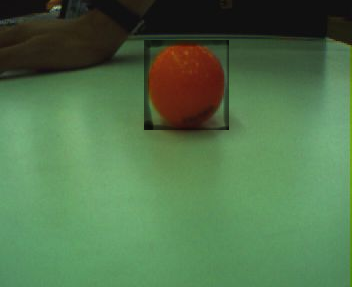
\includegraphics[width=5.5cm, height=3.5cm]{images/cam01.png}}

			\putat{150}{-90}{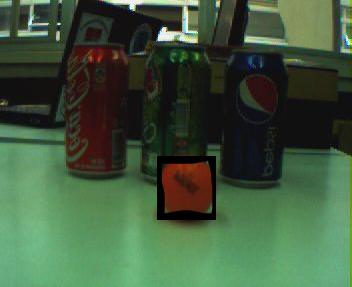
\includegraphics[width=5.5cm, height=3.5cm]{images/cam02.png}}

		}

		\subsection{Navegação}

		\frame{

			\frametitle{Exploração}

			\begin{itemize}

				\item O algoritmo de Exploração recebe as informações da função \textit{track-color} e toma a decisão de movimento do robô.

				\begin{itemize}

					\item Se a bola não foi localizada na imagem, girar para a esquerda.

					\item Senão, se o centróide está muito para a esquerda, girar para a direita.

					\item Senão, se o centróide está muito para a direita, girar para a esquerda.

					\item Senão, se o número de pixels for muito baixo, ir para a frente.

					\item Senão, parar.

				\end{itemize}

			\end{itemize}

		}
		
		\frame{

			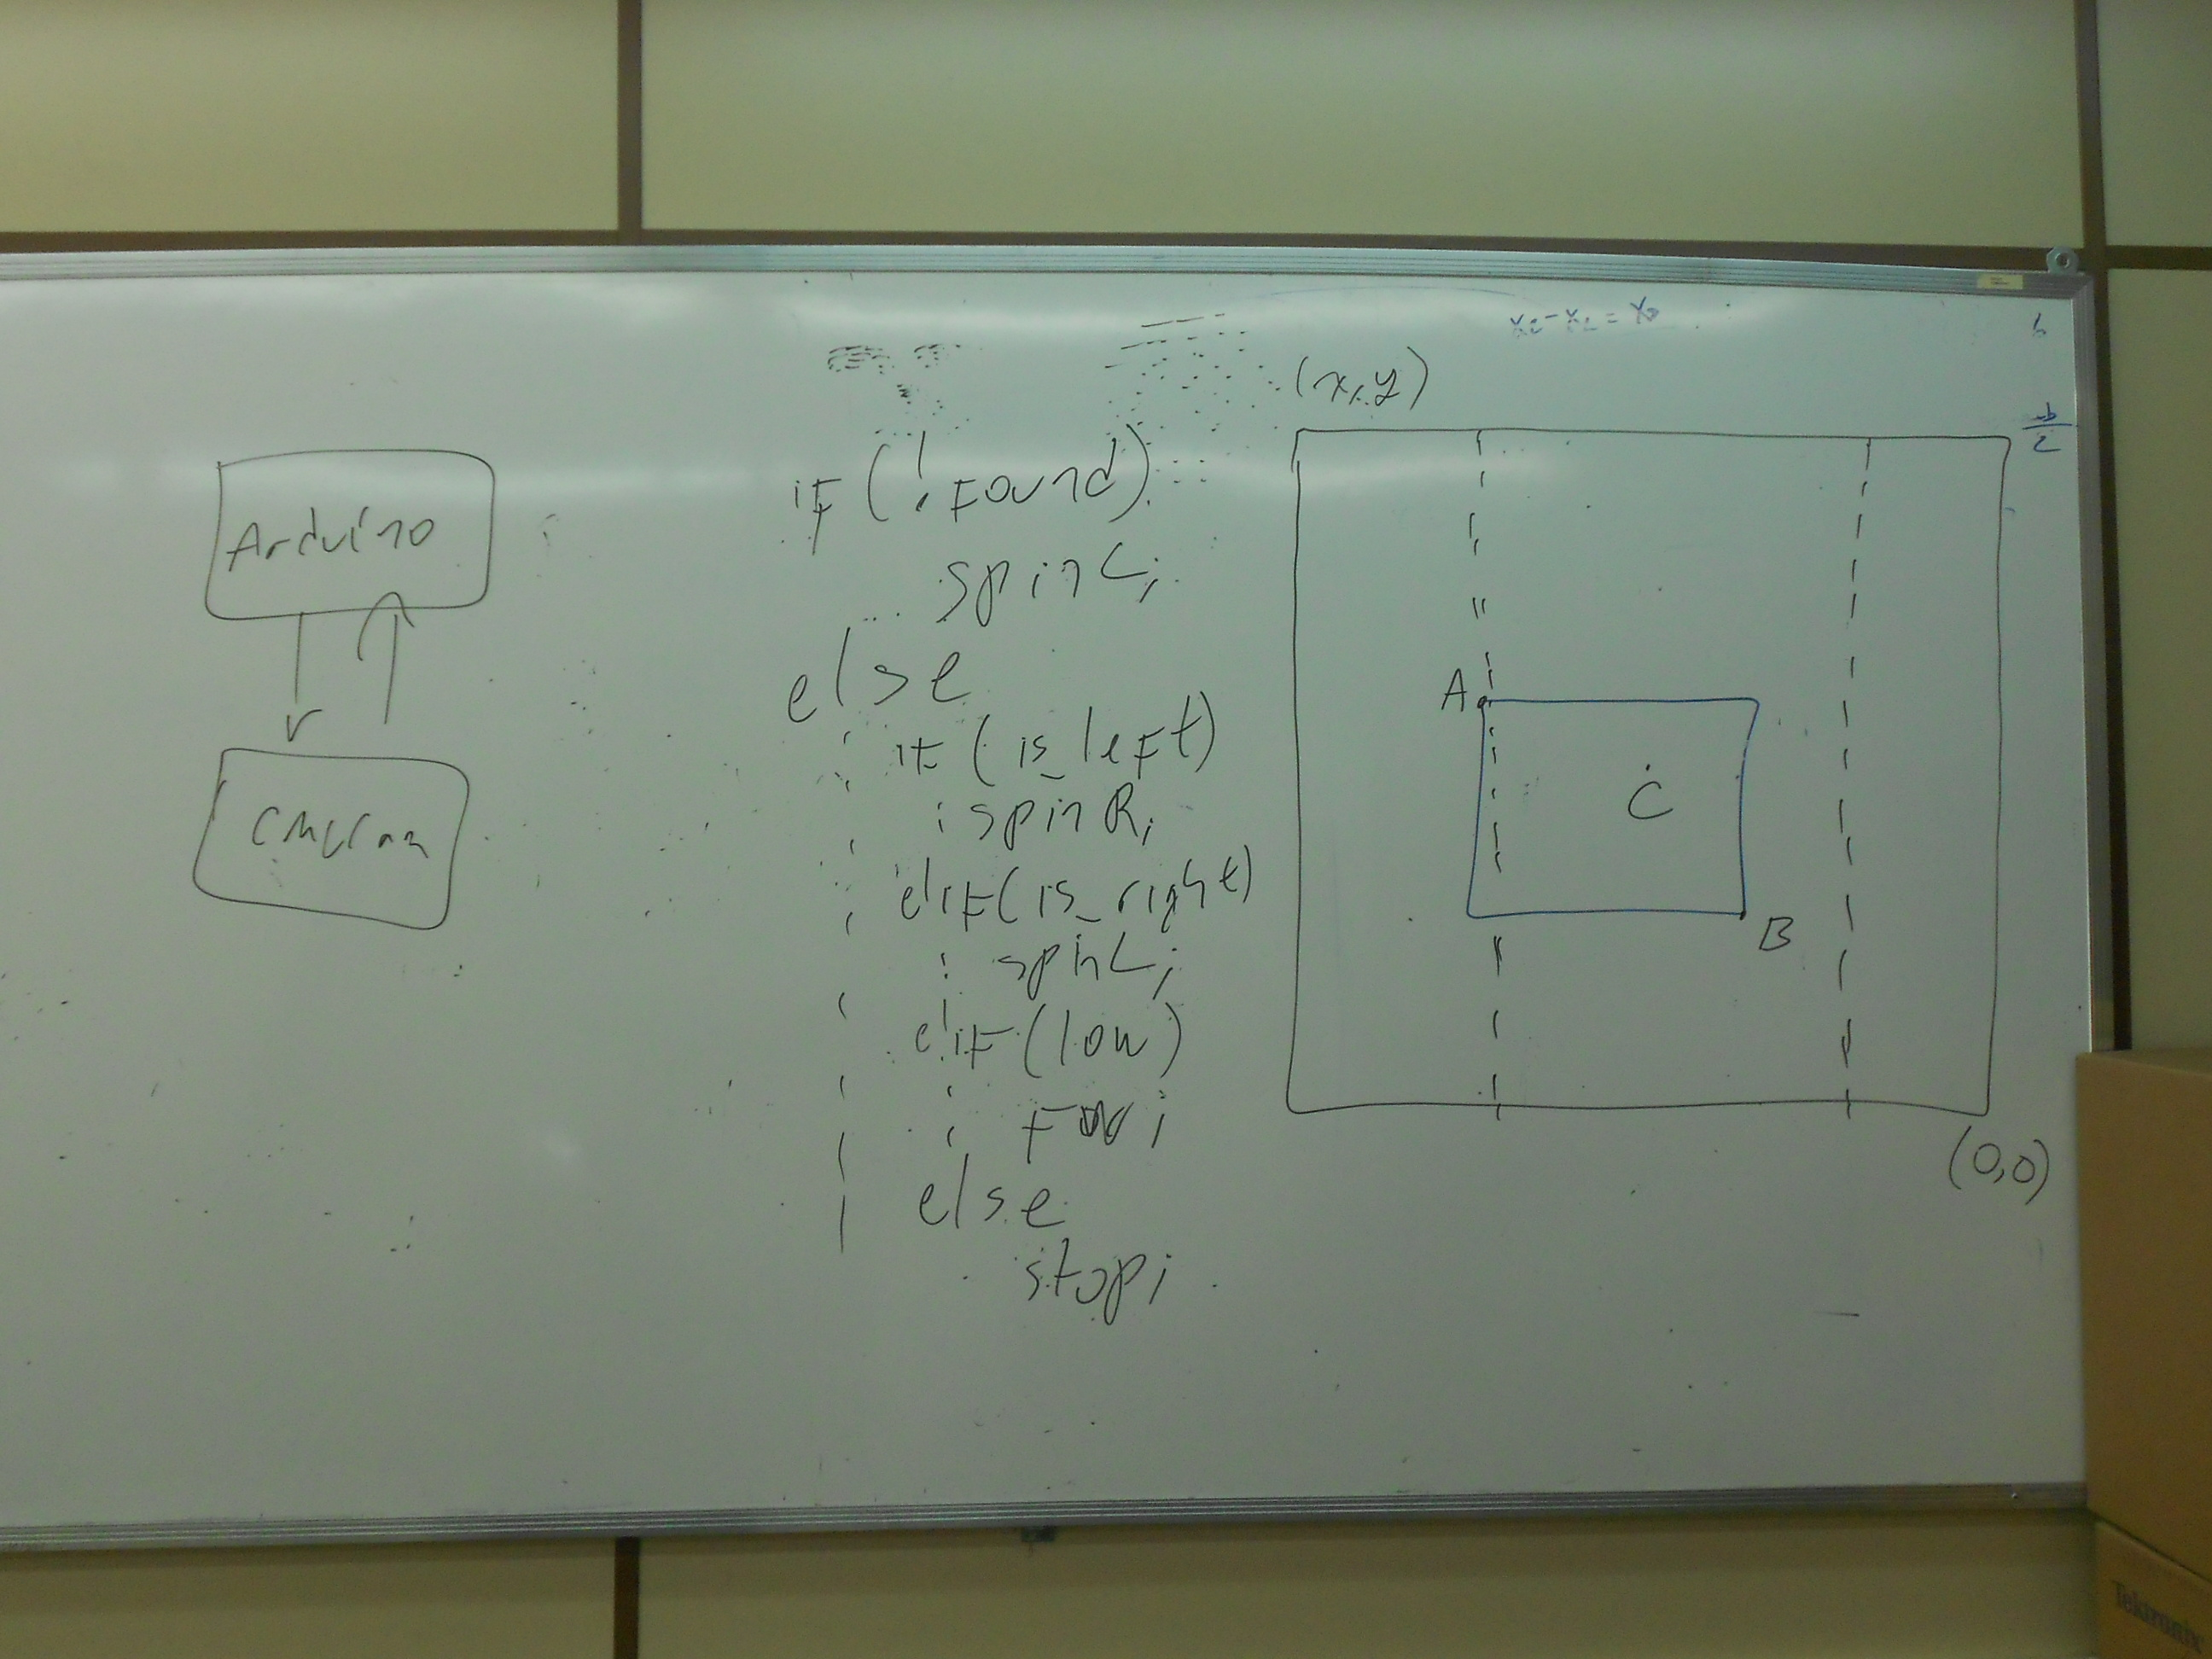
\includegraphics[width=11cm, height=7cm]{images/algoritmo}

		}

	\section{Conclusão}

		\frame{

			\frametitle{Dificuldades Encontradas}

				\begin{itemize}

					\item \textit{CMUCam}

					\begin{itemize}

						\item Atraso com compra e entrega.

						\item Falta de Documentação.

						\item Falta de Suporte.

						\item Informações antigas, desatualizadas e/ou inexatas da comunidade.

					\end{itemize}

					\item Comunicação Serial entre Arduino e \textit{CMUCam}


				\end{itemize}

		}

		\frame{

			\frametitle{Conclusão}

			\begin{itemize}

				\item Os objetivos foram parcialmente atingidos.

				\item A integração da \textit{CMUCam} com o Robô foi subestimada pela equipe.

				\item Maior tempo de aprendizado do que o previsto.

				\item Ter o robô pronto viabilizou e agilizou o projeto.

				\item Utilizar os exemplos prontos da \textit{CMUCam} facilitou o trabalho.

				\item Foi legal!

			\end{itemize}
		
		}
	
		\frame {

			\frametitle{Projetos Futuros}

			\begin{itemize}

				\item Corrigir os "erros" de comunicação

				\item Refazer o sistema mecânico - cabos e disposição dos componentes.

				\item Integrar a bússola ao robô.

				\item Aprimorar o sistema de visão.

				\item Implementar a navegação inteligente.

			\end{itemize}
		}

	\section{}

		\frame{
		
			\frametitle{Agradecimentos}

			\begin{itemize}

				\item Professores Myriam Delgado, Hugo Vieira, Mário Sérgio de Freitas, Cesar Tacla, João Fabro, Celso Kaestner

				\item Colegas Bruno Meneguele, Fernando Padilha, Vinicius Arcanjo

				\item Colegas Claudio Akio, Kaya Sumire Abe, Lucas Paiva

				\item Marceneiros do Almoxarifado da UTFPR

			\end{itemize}
		
		}

		\frame{

			\begin{centering}

				Projeto disponível em:

				\vspace{1cm}

				\textit{http://github.com/matheusaraujo/oficina2-robocam}

				\vspace{1.5cm}

				\textbf{Boas Férias!}

			\end{centering}

		}



\end{document}
